\section{Theoretical Analysis}

In this section, the circuit shown in Figure \ref{fig:Circuit} is analysed
theoretically using both the Mesh Method and Nodal Method.

\label{sec:analysis}
\subsection {{Mesh Method}}
For the Mesh Method, circular currents are introduced in the different single meshes of the circuit as shown in \ref{fig:MeshAnalysis} and then the circuit is evaluated considering those new currents.

\begin{figure}[h] \centering
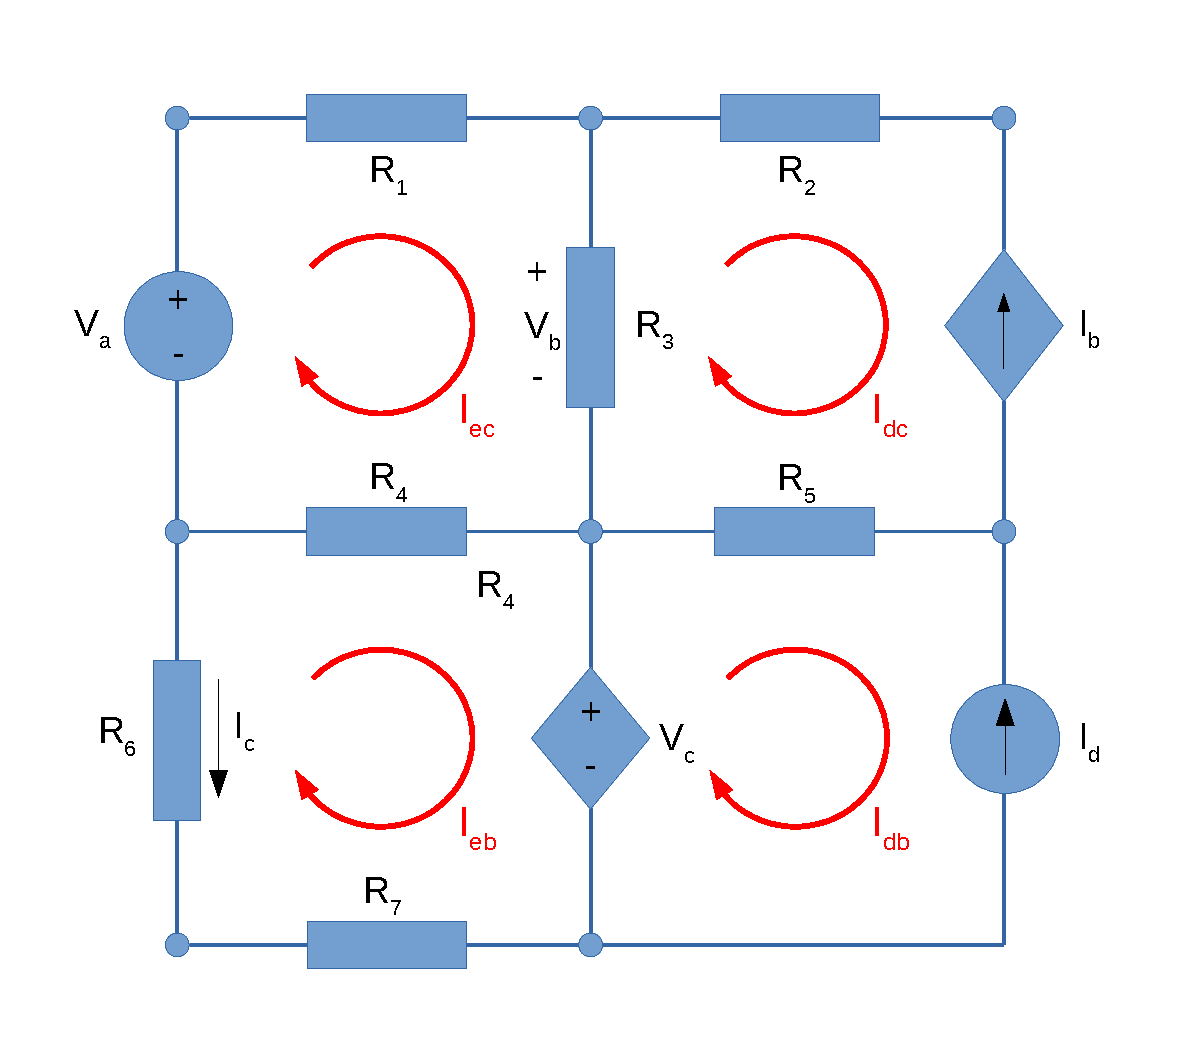
\includegraphics[width=0.4\linewidth]{MeshAnalysis.pdf}
\caption{Mesh Analysis}
\label{fig:MeshAnalysis}
\end{figure}

After identifying all the mesh currents, considering the above, it is now necessary to use Kirchhoff Voltage Law (KVL) in those meshes that don't contain current sources (Mesh EC (\textbf{\ref{eq:KVL_{ec}}}) and EB (\textbf{\ref{eq:KVL_{eb}}})) and relate the mesh currents to those imposed by the sources (Mesh DC (\textbf{\ref{eq:KVL_{dc}}}) and DB (\textbf{\ref{eq:KVL_{db}}}).

\vspace{0.1cm}

\begin{equation}
 -V_{a} + R_{1} I_{ec} + V_{b} + R_{4} (I_{ec} - I_{eb}) = 0
 \label{eq:KVL_{ec}}
\end{equation}

\begin{equation}
    I_{dc} = -I_{b}
    \label{eq:KVL_{dc}}
\end{equation}

\begin{equation}
     I_{db} = -I_{d}
     \label{eq:KVL_{db}}
\end{equation}

\begin{equation}
     V_{c} + R_{7} I_{eb} + R_{6} I_{eb} + R_{4} (I_{eb} - I_{ec}) = 0
      \label{eq:KVL_{eb}}
\end{equation}

\vspace{0.1cm}
Analysing the equations it is noticeable that we have 8 variables and that we'll need four more equations to solve the circuit. It is, also, important to notice that two of them are already given:
\begin{equation}
    V_{c} = K_{c} I_{c}
\end{equation}

\begin{equation}
    I_{b} = K_{b} V_{b}
\end{equation}

\vspace{0.1cm}
The other two are trivial equations found by the careful examination of the circuit with Ohm's Law:
\vspace{0.1cm}
\begin{equation}
    I_{c} = -I_{eb}
\end{equation}

\begin{equation}
    V_{b} = R_{3} (I_{ec} - I_{dc})
\end{equation}

\pagebreak
In the following table, both current and voltage for each component are presented:
\begin{center}
\begin{tabular}{ |c|c|c| }
 \hline
\textbf{Name} & \textbf{Current (A)} & \textbf{Tension (V)} \\
 \hline
 $I_{EC}$ & 2.143086e-04 & - \\ \hline 
$I_{DC}$ & 2.241280e-04  & -\\ \hline 
$I_{DB}$ & -1.024396e-03  & -\\ \hline 
$I_{EB}$ & -9.691453e-04  & -\\ \hline 
$V_{b}$ & - & -3.068815e-02 \\ \hline 
$V_{c}$ & - & 7.881834e+00 \\ \hline 
$I_{b}$ & -2.241280e-04  & -\\ \hline 
$I_{c}$ & 9.691453e-04  & -\\ \hline 

\end{tabular}
\end{center}

\subsection{Nodal Metod}
To determine the values of the current and voltage using the Nodal Method it is first necessary 
to find all the knots in the circuit, as shown in \ref{fig:NodeAnalysis}.

\begin{figure}[h] \centering
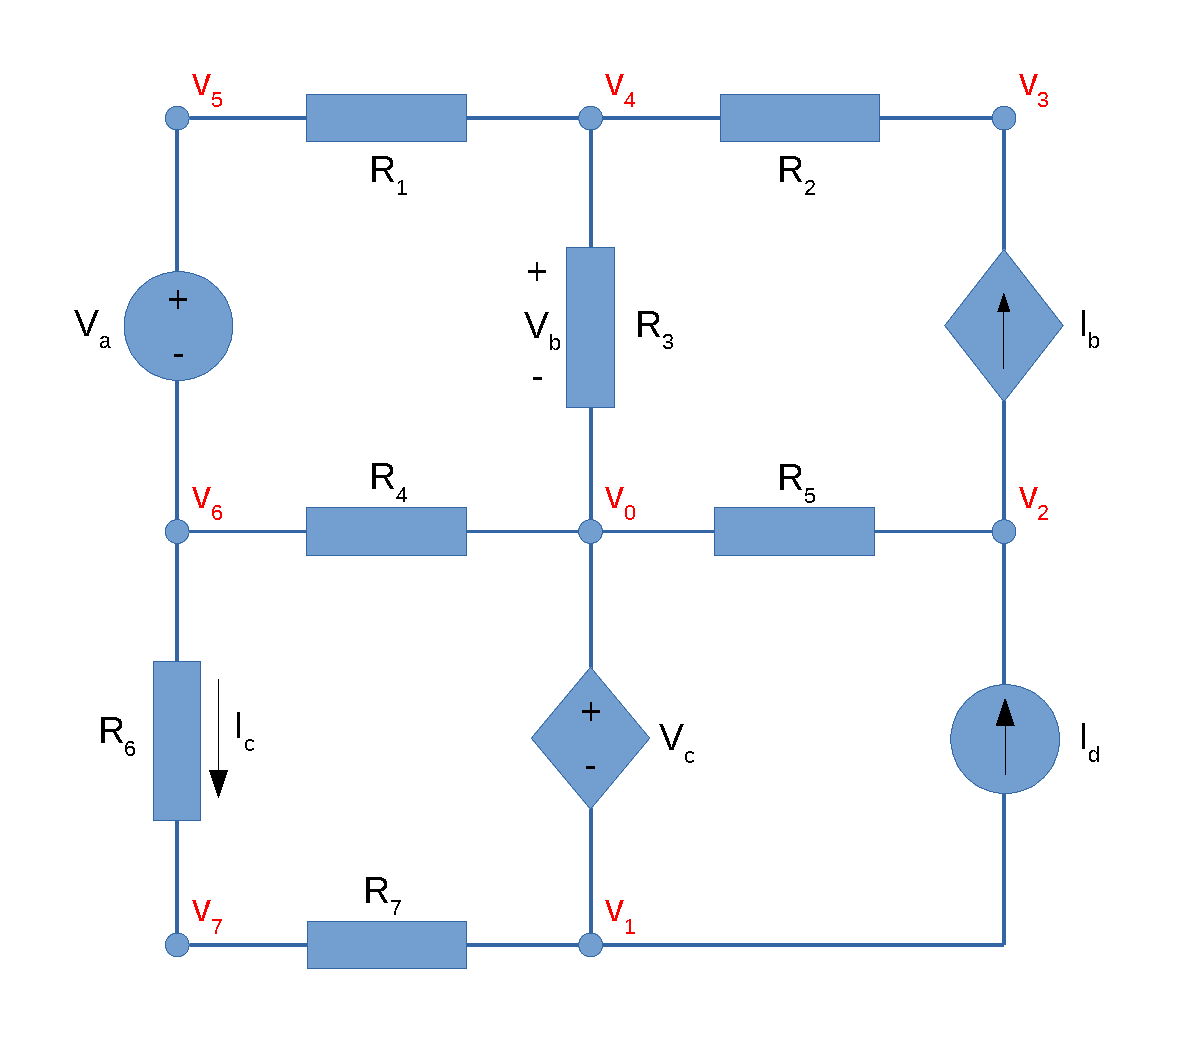
\includegraphics[width=0.4\linewidth]{NodeAnalysis.pdf}
\caption{Node Analysis}
\label{fig:NodeAnalysis}
\end{figure}


The Kirchhoff Current Law (KCL) is then used in the nodes that are not connected
to voltage sources (from \ref{eq:KCL_{9}} to \ref{eq:KCL_{12}})
\vspace{0.1cm}
\begin{equation}
    V_{5} G_{1} - V_{4} (G_{1} + G_{2}) + V_{3} G_{2} - V_{b} G_{3} = 0
    \label{eq:KCL_{9}}
\end{equation}

\begin{equation}
    -V_{3} G_{2} + V_{4} G_{2} + I_{b} = 0
\end{equation}

\begin{equation}
    V_{2} G_{5} + V_{0} G_{5} + I_{d} = I_{b}
\end{equation}

\begin{equation}
    G_{6} (V_{6} - V_{7}) - I_{c} = 0
    \label{eq:KCL_{12}}
\end{equation}
\vspace{0.5cm}

\pagebreak

In \ref{eq:KCL_{13}} and \ref{eq:KCL_{14}}, a relationship is established between
a knot's voltage and the voltage sources that are connected to them:

\begin{equation}
    V_{5} - V_{6} = V_{a}
    \label{eq:KCL_{13}}
\end{equation}

\begin{equation}
    V_{c} = V_{0} - V_{1}
    \label{eq:KCL_{14}}
\end{equation}



\vspace{0.5cm}

By analysing the circuit we get:

\vspace{0.5cm}
\begin{equation}
    V_{c} = K_{c} I_{c}
\end{equation}

\begin{equation}
    I_{b} = K_{b} V_{b}
\end{equation}

\begin{equation}
    V_{b} = V_{4} - V_{0}
\end{equation}

\begin{equation}
    V_{0} = 0
\end{equation}


Using Ohm's Law:

\begin{equation}
    I_{c} = V_{6} G_{6} - V_{7} G_{6}
\end{equation}
\vspace{0.5cm}


The continuity of current in voltage sources allows to write this equation:
\begin{equation} 
    V_{5} G_{1} - V_{4} G_{1} + I_{c} + V_{0} G_{4} - V_{6} G_{4} = 0   
\end{equation}

In the following table, both current and voltage for each component are presented:
\begin{center}
\begin{tabular}{ |c|c|c| }
 \hline
\textbf{Name} & \textbf{Current (A)} & \textbf{Tension (V)} \\
 \hline
 $v_{0}$ & 0.000000e+00 \\ \hline 
$v_{1}$ & -7.881834e+00 \\ \hline 
$v_{2}$ & 3.805553e+00 \\ \hline 
$v_{3}$ & -4.970348e-01 \\ \hline 
$v_{4}$ & -3.068815e-02 \\ \hline 
$v_{5}$ & 1.871742e-01 \\ \hline 
$v_{6}$ & -4.894946e+00 \\ \hline 
$v_{7}$ & -6.897288e+00 \\ \hline 
$V_{b}$ & -3.068815e-02 \\ \hline 
$V_{c}$ & 7.881834e+00 \\ \hline 
$I_{b}$ & -2.241280e-04 \\ \hline 
$I_{c}$ & 9.691453e-04 \\ \hline 

\end{tabular}
\end{center}

\pagebreak





